\section{Training Dynamics}

In this section, we study the trajectories $\bm z(t)$ that are solutions of the two gradient flow equations \eqref{eq:kernel_gf} and \eqref{eq:adaptive_gf} corresponding to the kernel and adaptive regimes. 
%We analyze these in case where the number of neurons is infinite ($m = \infty$)


\subsection{Kernel Learning}

\note{This section needs more work} 
\note{We should point out that minimizing $\|c\|$ minimizes curvature for the uniform initialization, because this is a generally useful fact}

We first consider the dynamics of kernel learning in the limit when the number of neurons is infinite ($m = \infty$). In this regime, we only train the outer layer paramters $\bm c$. In phase space, this corresponds to neuron trajectories that move radially away from the origin (see Figure \ref{fig:trajectories}). In this setting, it is convenient to reparameterize our model as

\begin{equation}\label{eq:infinite_model}
    f_{\bm \theta}(x) = \int c_+(s) a_+(s)[x-s]_+ ds \, + \,  \int c_-(s) a_-(s)[s-x]_+ ds
\end{equation}

where $a_+, a_-, c_+, c_-$ are scalar functions corresponding to the distributions of positive and negative neurons \note{Joan, how should we argue that this is a valid way to go to the limit? It should be because we can integrate over scalings of $a, b$ without chaning loss or dynamics}
Use the scaling $1/\sqrt{m}$ and refer to prior work (NTK and Chizat, Bach), no need to redo the argument here. 

We introduce the following kernel
\begin{equation}
\begin{gathered}
    f(x) = \sum_{j=1}^s \alpha_j K(x_j, x) \text{ where } \\
    K(x, x') = \int a_+(s)^2[x - s]_+ [x' - s]_+ ds + \int a_-(s)^2[s - x]_+ [s - x']_+ ds\\
    = \int_{-\infty}^{\min x, x'} a_+(s)^2 (x - s)(x' - s) ds + \int_{\max x, x'}^\infty a_-(s)^2(s - x) (s - x')_+ ds.
\end{gathered}
\end{equation}

In the overparameterized case, we wish to solve least squares problem

\begin{equation}\label{eq:least_squares_op}
    \text{minimize } \|\bm c\|^2 \text{ s.t. } f_{\bm \theta}(\bm x) = \bm y.
\end{equation}

Solutions $f(x)$ can be written in terms of the kernel as

\begin{equation}~\label{eq:kernel_solution}
    \hat f(x) = \sum_{j=1}^s \alpha_j K(x_j,x),
\end{equation}

where $\alpha_j = K^{-1}(\bm y)$ and $K(x_i, x_j) = (\bm K_{c})_{ij}$. We note that the gradient flow will actually converge to this solution only if $\bm c(0)$ is initialized sufficiently close to the origin. Contrary to to the usual kernels considered in ReLU networks~\cite{cho2009kernel,bach2017breaking}, which consider neurons uniformly distributed over a sphere, it is natural in our setting to consider \emph{unform distributions} of neurons $a_+(s) = \mathds 1[k_0,k_1]$ (neurons with $a=1$ uniformly distributed in $[k_0, k_1]$) or $a_+(x) = a_-(s) = \mathds 1[k_0,k_1]$ (neurons with $a=1$ and $a=-1$ uniformly distributed in $[k_0, k_1]$). Interestingly, we note that these distributions of neurons lead to \emph{cubic spline interpolation}.

\begin{proposition} If $a_+(s) = \mathds 1[k_0,k_1]$ or $a_+(x) = a_-(s) = \mathds 1[k_0,k_1]$, the kernel $K(x,x')$ is a piecewise cubic polynomial in $x$ and $x'$. In particular, in the overparameterized setting, the solution~\eqref{eq:kernel_solution} will be an interpolating \emph{cublic spline}.
\end{proposition}

Another way to justify this result is to notice that if $f_{\bm \theta}$ is as in~\eqref{eq:infinite_model} with $a_+(x)$, then $f_{\bm \theta}''(x) = c_+(s)$. Hence, the interpolation is minimizing \emph{curvature}.
We remark that machine learning packages such as PyTorch use a uniform distribution for linear layer parameter initialization by default.
We verify that indeed, solutions to \eqref{eq:leastsquares} converge to cubic splines as $m$ grows in Figure~\ref{fig:cubic_splines}. We also point out that in Kernel Learning, early termination of gradient flow acts as a regularizer favoring smooth, non-interpolatory solutions (see \cite{NTKJacot} and Section~\ref{sec:implicit_regularizer}).



\subsection{Active Learning}

We now consider the dynamics of adaptive learning. In this regime, we train all network parameters, and reparameterize the model as 

%we only train the inner layer parameters $\bm a, \bm b$. In phase, space this corresponds to neuron trajectories which move along a piecewise constant gradient field  with boundaries corresponding to the boundaries of the activation regions, $R$ \eqref{eq:activatioon_region}.
%In this regime, it is convenient to 

\begin{equation}
    f_\mathbf{z}(x) = \frac{1}{m}\sum_{i=1}^m c_i \langle \tilde{x}, \theta_i \rangle_+~,
\end{equation}
with parameters $\mathbf{z}=(z_1\dots z_m)$, $z_i=(c_i ,\theta_i) \in \mathbb{R} \times S^1$, and  
where $\tilde{x} = (x, 1)$. %\bm v(\theta) \in S^1 = (\cos(\theta), \sin(\theta))$, and $\langle \cdot, \cdot \rangle_+$ is a ReLU. 
Thanks to the homogeneity of the ReLU activation function, this parametrisation represents the same functional space as the model using the standard parameterization (\ref{eq:standard_parameterization}).
We use the scaling in $1/m$ in order to obtain an asymptotic behavior as $m\to \infty$ whereby both first and second layer weights 
move away from their initialization under gradient descent and the kernel dynamics no longer apply-- the \emph{active learning} regime of \cite{chizat2018note}. 

Using this normalization, and following the mean-field formulation of single-hidden layer neural networks of \cite{meimontanari, chizat2018global, rotskoffeve}, we express the function as an expectation with respect to a probability measure $\mu$ over the cylinder $\mathcal{D} = \mathbb{R} \times S^1$:
\begin{equation}
    f_\mathbf{z}(x) = \int_\mathcal{D} \varphi(z;x) \mu^{(m)}(dz)~,
\end{equation}
where $\varphi(z;x):=c \langle \tilde{x}, \theta_i \rangle_+$ and $\mu^{(m)}(z) = \frac{1}{m} \sum_{i=1}^m \delta_{z_i}(z)$ 
is the empirical measure determined by the $m$ particles $z_i$, $i=1\dots m$.
The least squares loss in this case becomes 
\begin{eqnarray}
    L(\mathbf{z}) &=& \frac{1}{2}\| f_\mathbf{z} - y \|_\mathcal{X}^2 \\
    &=& \frac{1}{2}\| y\|^2_\mathcal{X} - \langle f_\mathbf{z} , y \rangle_\mathcal{X} + \frac{1}{2}\| f_\mathbf{z} \|^2_\mathcal{X} \\
    &=& C_y - \frac{1}{m} \sum_{i=1}^m \langle \varphi_{z_i} , y \rangle_\mathcal{X} + \frac{1}{2m^2} \sum_{i,i'=1}^m \langle \varphi_{z_i} ,\varphi_{z_{i'}} \rangle_\mathcal{X} ~,
\end{eqnarray}
where $\langle f, g \rangle_\mathcal{X} := \sum_{j=1}^s f(x_j) g(x_j)$ is the empirical dot-product. 
This loss may be interpreted as the Hamiltonian of a system of $m$-interacting particles, under external 
field $F$ and interation kernel $K$ defined respectively by 
\begin{equation}
F(z):= \langle \varphi_z, y \rangle_\mathcal{X} ~,~K(z, z'):= \langle \varphi_{z} ,\varphi_{z'} \rangle_\mathcal{X}~.    
\end{equation}
We may also express this Hamiltonian in terms of the empirical measure, by abusing notation
$$L(\mu^{(m)}) = C_y - \int_\mathcal{D} F(z) \mu^{(m)}(dz) + \frac{1}{2} \iint_{\mathcal{D}^2} K(z,z') \mu^{(m)}(dz) \mu^{(m)}(dz')~.$$

A direct calculation shows that the gradient $\nabla_{z_i} L(\mathbf{z})$ can be written as 
$$\frac{m}{2} \nabla_{z_i} L(\mathbf{z}) = \nabla_z V(z_i; \mu^{(m)})~,$$%\text{ with } $$
where $V$ is the potential function 
\begin{equation}
\label{eq:potential}
    V(z;\mu):= -F(z) + \int_\mathcal{D} K(z, z') \mu(dz')~.
\end{equation}
The gradient flow in the space of parameters $\mathbf{z}$ can be now interpreted in terms of a gradient flow in the space of measures over $\mathcal{D}$ by using the notion of Wasserstein gradient flows \cite{meimontanari, chizat2018global, rotskoffeve}. Indeed, 
equation \ref{eq:potential} shows that particles evolve in $\mathcal{D}$ by ``feeling" a velocity field $\nabla V$ defined in $\mathcal{D}$. 
This formalism allows us now to describe the dynamics independently of the number of neurons $m$, by replacing the empirical measure $\mu^m$ 
by any generic probability measure $\mu$ in $\mathcal{D}$. The evolution of a measure under a generic time-varying vector field is given by the 
so-called continuity equation:
\begin{equation}
\label{eq:continuity}
    \partial_t \mu_t = \mathrm{div} ( \nabla V \mu_t)~,
\end{equation}
understood in the weak sense, ie 
$\partial_t \left(\int_\mathcal{D} \phi(z) \mu_t(dz)\right) = - \int \langle \nabla \phi(z), \nabla V(z;\mu_t) \rangle \mu_t(dz)$, 
$\forall \phi \in C^1_c(\mathcal{D})$ continuously differentiable and with compact support. The global 
convergence of this PDE for interaction kernels arising from single-hidden layer neural networks has been 
 established under mild assumptions in \cite{meimontanari, chizat2018global, rotskoffjoan}. Although 
 the conditions for global convergence hold in the mean field limit $m \to \infty$, a propagation-of-chaos 
 argument from statistical mechanics gives Central Limit Theorems for the behavior of finite-particle systems 
 as fluctuations of order $1/\sqrt{m}$ around the mean-field solution; see \cite{rotskoffeve, rotskoffjoan} for further details. 

The dynamics in $\mathcal{D}$ are thus described by the velocity field $\nabla V(z; \mu_t)$, which depends on the current 
state of the system through the measure $\mu_t(z)$, describing the probability of encountering a particle
at position $z$ at time $t$. We emphasize that equation (\ref{eq:continuity}) is valid 
for any measure, including the empirical measure $\mu^{(m)}$, and is therefore an exact model for 
the dynamics in both the finite-particle and infinite-particle
regime. Let us now describe its specific form in the case of the empirical loss given above. 

Assume without loss of generality that the datapoints $x_j \in \mathbb{R}$, $j\leq s$ satisfy $x_j \leq x_{j'}$ whenever $j < j'$.
Denote 
$$\mathcal{C}_j := \{ j' ; j' \leq j\} \text{ for } j=1\dots s,~\mathcal{C}_{s+j} := \{ j' ; j' > j \},\text{ for }j=1\dots s-1~.$$
We verify that for each $j$, the angles $\alpha_j = \arctan(x_j) \pm \pi/2$ partition the circle $S^1$ into $2s-1$ regions $\mathcal{A}_k$, 
which are in one-to-one correspondence with the sets $\mathcal{C}_k$, in the sense that 
$$\theta \in \mathcal{A}_k \Longleftrightarrow \{j ; \langle \tilde{x}_j , \theta \rangle \geq 0 \} = \mathcal{C}_k~.$$
\note{(These are the same as $R(\bm \tau)$ defined above, let's make the notation consistent)}
We also denote by $\mathcal{B}_j$ 
%$\mathcal{B}_j = \{ \theta; \theta \in (\alpha_j - \pi/2, \alpha_j+\pi/2)\}$ for $j=1\dots s$
the half-circle where $\langle \tilde{x}_j, \theta\rangle \geq 0$. Let $t(\theta)$ be the tangent vector of $S^1$ at $\theta$.

Let $z=(c,\theta)$, and suppose $\theta \in \mathcal{A}_k$. From (\ref{eq:potential}), the angular velocity field $\nabla_\theta V(z; \mu_t)$ is given by 
\begin{eqnarray}
\label{eq:meanfield1}
    \nabla_\theta V(z; \mu_t) &=& -\nabla_\theta F(z) + \int_\mathcal{D} \nabla_\theta K(z, z') \mu_t(dz') \nonumber \\
    &=& -c\left( \sum_{j \in \mathcal{C}_k} y_j \langle \tilde{x}_j, t(\theta)\rangle  -\int_\mathcal{D} c'\sum_{j \in \mathcal{C}_k} \langle \tilde{x}_j,t(\theta)\rangle \langle \tilde{x}_j, \theta' \rangle_+ \mu_t(dc', d\theta') \right) \nonumber \\
    &=& -c \sum_{j \in \mathcal{C}_k} \langle \tilde{x}_j, t(\theta)\rangle \left(y_j - \int_{\mathbb{R} \times \mathcal{B}_j} c' \langle \tilde{x}_j, \theta' \rangle \mu_t(dc', d\theta') \right) \nonumber \\
    &=& c \left \langle \sum_{j \in \mathcal{C}_k} r_j(t) \tilde{x}_j, t(\theta) \right \rangle~,
\end{eqnarray}
where 
$$r_j(t) = f_{\mu_t}(x_j) - y_j =    \int_{\mathbb{R} \times \mathcal{B}_j} c \langle \tilde{x}_j,\theta  \rangle \mu_t(dc, d\theta)  - y_j$$
is the residual at point $x_j$ at time $t$. 
Similarly, the field in the direction of the charges is given by
\begin{equation}
\label{eq:meanfield2}
    \nabla_c V(z; \mu_t) =  \left \langle \sum_{j \in \mathcal{C}_k} r_j(t) \tilde{x}_j, \theta \right \rangle ~.
\end{equation}
Equations (\ref{eq:meanfield1}, \ref{eq:meanfield2}) show that the dynamics are entirely controlled by the 
$s$-dimensional vector of residuals $\mathbf{r}(t)=(r_1(t), \dots r_s(t))$, and that the flow is piece-wise linear 
on each cylindrical region $\mathbb{R} \times \mathcal{A}_k$. 
Under the assumptions that ensure 
global convergence of (\ref{eq:continuity}), we have $\lim_{t \to \infty} L(\mu(t)) = 0$, 
and therefore $\| \mathbf{r}(t) \| \to 0$. The oscillations of $\mathbf{r}(t)$ as it converges 
to zero determine the relative orientation of the flow within each region. 

Observe that for each $j$, 
\begin{eqnarray}
\label{eq:oderesiduals}
\dot{r}_j(t) &=& \partial_t f_{\mu_t}(x_j) = \partial_t \left( \int_\mathcal{D} \varphi(z;x_j) \mu_t(dz) \right) \nonumber \\ 
&=& - \int_\mathcal{D} \langle \nabla_z \varphi(z;x_j), \nabla V(z;\mu_t) \rangle \mu_t(dz) \nonumber \\
&=& - \int_\mathcal{D} \left(  \nabla_\theta \varphi(z;x_j) \cdot \nabla_\theta V(z;\mu_t)  +  \nabla_c \varphi(z;x_j) \cdot \nabla_c V(z;\mu_t)  \right) \mu_t(dz) \nonumber \\
&=& -\sum_{k; \mathcal{A}_k \subset \mathcal{B}_j} \int_{\mathbb{R} \times \mathcal{A}_k} \left( c^2  \tilde{x}_j^\top (t(\theta)t(\theta)^\top) (\sum_{j' \in \mathcal{C}_k} r_{j'}(t) \tilde{x}_{j'}) + \tilde{x}_j^\top (\theta \theta^\top) (\sum_{j' \in \mathcal{C}_k} r_{j'}(t) \tilde{x}_{j'}) \right) \mu_t(dz) \nonumber  \\
&=& -\tilde{x}_j^\top \sum_{k; \mathcal{A}_k \subset \mathcal{B}_j}  \Sigma_k(t) (\sum_{j' \in \mathcal{C}_k} r_{j'}(t) \tilde{x}_{j'})~, 
\end{eqnarray}
where 
$$\Sigma_k(t) = \int_{\mathbb{R} \times \mathcal{A}_k} \left(c^2 t(\theta)\, t(\theta)^\top + \theta\, \theta^\top\right) \mu_t(dc,d\theta) $$
tracks the covariance of the measure along each 
cylindrical region. Equation (\ref{eq:oderesiduals}) 
defines a system of ODEs for the residuals $\mathbf{r}(t)$, but its coefficients are time-varying, and behave roughly as quadratic terms in $\mathbf{r}(t)$ (since they are second-order moments of the measure whereas the residuals are first-order moments). It may be possible to obtain asymptotic control of the oscillations $\mathbf{r}(t)$ by applying Duhamel's principle, 

Although the analytical solution of the PDE and ODE above is out of the scope of this work, we can use the flow equations above to argue qualitatively that the dynamics are now fundamentally different than in the kernel regime, 
and in particular they become \emph{data-adaptive}. In the cylindrical parametrisation, the kernel dynamics 
only move the charges, thus the angular distribution $\bar{\mu}(\theta) = \int_\mathbb{R} \mu(dc, \theta)$ equals the initial distribution 
and does not adapt to the input data. 

Let $z=(c,\theta)$ with $\theta$ at a boundary of two regions $\mathcal{A}_k$, $\mathcal{A}_{k+1}$. The velocity field is modified at the transition  by 
$$
\nabla V(z)\lvert_{\mathcal{A}_k} - \nabla V(z)\lvert_{\mathcal{A}_{k+1}} = r_{j*}(t) \left( 
\begin{array}{c}
c  \langle \tilde{x}_{j*}, t(\theta) \rangle \\
\langle \tilde{x}_{j*}, \theta \rangle
\end{array}\right)
~,$$
where $j_*$ is such that $\langle \tilde{x}_{j*}, \theta \rangle =0$ since $\theta$ is at the boundary of $\mathcal{A}_k$. It follows that the only discontinuity is in the angular direction, of magnitude $|c\, r_{j*}(t)|$, since $|\langle \tilde{x}_{j*}, t(\theta) \rangle| =1$.

An interesting phenomena arises when the angular components of $\nabla V(z)\lvert_{\mathcal{A}_k}$ and $\nabla V(z)\lvert_{\mathcal{A}_{k+1}}$ have opposite signs, corresponding to an `attractor' (resp `repulsor') that attracts/repels particles along the direction given by $\tilde{x}_{j*}$. By denoting $\alpha_k = \left \langle \sum_{j \in \mathcal{C}_k} r_j(t) \tilde{x}_j, t(\theta) \right \rangle$, from (\ref{eq:meanfield1}) we deduce that this occurs when
\begin{equation}
 \left|  \alpha_k \right| < |r_{j*}(t)| \text{ and } \text{sign}(\alpha_k) \neq \text{sign}(r_{j*}(t))~.    
\end{equation}
In words, mass will concentrate towards input points where the residual is currently large and of opposite sign from a weighted average of neighboring residuals. This is in stark contrast with the kernel dynamics, where there is no adaptation to the input datapoints. 


%Let $\mathbf{M} $




% The gradient flow in this parameterization is

% \begin{equation}
%     \begin{bmatrix}
%         c_i'(t)\\
%         \theta_i'(t)
%     \end{bmatrix} = 
%     \begin{bmatrix}
%         \sum_{j=1}^s =  
%     \end{bmatrix}
% \end{equation}
% regime where\theta'(t) $\delta_i \ll \|  = \xi_i \|$. In this regime, neurons move parallel to the reduced gradient field $\nabla \tilde{L}(\bm \xi)$ (see Figure \ref{fig:trajectories}). These trajectories are equivalent to those when training only the bottom layer parameters $(\bm a, \bm b)$ while keeping the top layer ($\bm c$) fixed. To understand the dynamics in this regime, we write the function $f$ in terms of the reduced parameters

% \begin{equation}
%     f_{\bm \xi}(x) = \sum_{i=1}^m \langle (x, 1), (u_i, v_i) \rangle_+ 
% \end{equation}

% The gradient of the loss with respect to the reduced parameters is 
% \begin{equation}\label{eq:grad_reduced}
%     \nabla \tilde{L}(\bm \xi)_i = \sum_{i=1}^s (f_{\bm \xi}(x_j) - y_j) \epsilon_i \tau_{ij} \begin{bmatrix}x_j \\ 1\end{bmatrix} 
% \end{equation}



% which is a piecewise constant function with the boundary between pieces occuring along the sample lines $u x_j + v = 0, j = 1 \ldots s$ (see Figure~\ref{fig:reduced_grad}). While the gradient field is in general discontinuous on the boundary of a sample, the component along a sample line is continuous







\subsection{Mixed Learning: Interpolating Kernel and Adaptive Learning}

In practice, the dynamics of gradient flow are a combination of the Kernel and Adaptive regimes. We can understand how much each regime contributes to the dynamics by considering the following conserved quantity:

\begin{lemma} \label{le:fixed_delta}
If $\bm \theta(t) = (\bm a(t), \bm b(t), \bm c(t))$ is a solution of the gradient flow \eqref{eq:gradient_flow}, then the quantities
\begin{equation}\label{eq:invariants}
\bm \delta = (\delta_i = c_i(t)^2 - a_i(t)^2 - b_i(t)^2)_{i=1}^m
\end{equation}
remain constant for all $t$. In particular, given a phase representation of a neuron $(\epsilon_i, u_i,v_i) = (\text{sign}(c_i), |c_i|a_i,|c_i|b_i)$, we can uniquely recover the original neuron $(a_i,b_i,c_i)$ since
\begin{equation}\label{eq:c_uv}
    c_i^2 = \frac{\delta_i + \sqrt{\delta_i^2 + 4 (u_i^2 + v_i^2)}}{2}. 
\end{equation}
\end{lemma}

Lemma~\ref{le:fixed_delta} allows us to analyze the dynamics in phase space without loss of generality. We can thus write the function and loss in phase space

\begin{equation}
    \tilde{f}_{\bm \xi}(x) = \sum_{j=1}^m \epsilon_i [ u_i x + v_i]_+.
\end{equation}
\begin{equation}
    \tilde L(\bm \xi) = \sum_{i=1}^s |\tilde{f}_{\bm \xi}(x_i) - y_i|^2, \qquad \bm \xi = (\bm \epsilon, \bm u, \bm v),  
\end{equation}

and consider the evolution of the parameters $\bm u$ and $\bm v$ during gradient flow. Note that so long as the signs, $\epsilon_i$ stay fixed, the trajectories of $\bm u$ and $\bm v$ will allow us to understand the trajectories of $\bm a$, $\bm b$ and $\bm c$. In that sense, the analysis here is \emph{local} within a time window with fixed $\epsilon$.

\begin{theorem}\label{thm:reduced_parameter_grad}
Let $\bm \theta(t)$ be an integral curve for the gradient flow \eqref{eq:gradient_flow} of $L(\bm \theta)$, and let $\bm \delta = (\delta_i) \in \RR^m$ be the vector of invariants~\eqref{eq:invariants}, which depend only on the initialization $\bm \theta(0)$. If $\bm \xi(t) = (\bm \epsilon, \bm u(t), \bm v(t))$ is curve of reduced parameters corresponding to $\bm \theta(t)$, then we have that
\begin{equation}
\begin{bmatrix}
u_i'(t)\\
v_i'(t)
\end{bmatrix} =
\bm P_{\delta_i}(u_i,v_i)
\begin{bmatrix}
\nabla_{u_i} \tilde L (\bm \xi)\\
\nabla_{v_i} \tilde L (\bm \xi)\\
\end{bmatrix},
\quad i=1,\ldots,m,
\end{equation}
where
\begin{equation}\label{eq:neuron_kernel}
\bm P_\delta(u_i,v_i) = \begin{bmatrix}
    a_i^2 + c_i^2  & 
    a_i b_i        \\
    a_i b_i               & 
    b_i^2 + c_i^2\\
\end{bmatrix} = 
\begin{bmatrix}
\frac{u_i^2}{c(u_i, v_i)^2} + c(u_i, v_i)^2 & \frac{u_i v_i}{c(u_i, v_i)^2}\\
\frac{u_i v_i}{c(u_i, v_i)^2} &  \frac{v_i^2}{c(u_i, v_i)^2} + c(u_i, v_i)^2\\
\end{bmatrix},
\end{equation}

and $c(u_i, v_i)^2 = \frac{\delta_i + \sqrt{\delta_i^2 + 4 (u_i^2 + v_i^2)}}{2}$
\end{theorem}

It is easy to verify that the eigenvalue-eigenvector pairs of $\bm P_{\delta_i}(u_i,v_i)$ are
\begin{align}
    (\lambda_1, \bm w_1) &= (a_i^2+ b_i^2 + c_i^2, (u_i,v_i))
    \label{eq:radial_eigenval}\\
    (\lambda_2, \bm w_2) &= (c_i^2, (-v_i,u_i)) 
    \label{eq:tangential_eigenval}
\end{align}
which define two types of trajectories. We can understand the dynamics of a neuron as a mix between these two types. In fact, writing $\rho_i = u_i^2 + v_i^2$, it is straightforward to verify that:

\begin{itemize}
    \item If $\rho_i \ll |\delta_i|$ and $\delta < 0$, then the eigenvector $\bm w_1$ dominates and $\xi'(t) \propto \xi$ causing the neuron moves \emph{radially} in phase space.
    \item If $\rho_i \ll |\delta_i|$ and $\delta > 0$, then the eigenvector $\bm w_2$ dominates and $(\dot u_i(t), \dot v_i(t)) \propto \nabla_{u_i} \tilde L(\bm \xi(t))$, causing the neuron to parallel to the vector field $\nabla \tilde L(\bm \xi)$.
\end{itemize}

Figure~\ref{fig:trajectories} shows the trajectories corresponding to different values of $\delta_i$ for a neuron. The extreme cases of $\delta = -\infty$ and $\delta = +\infty$ correspond exactly to the Kernel and Adaptive regimes respectively. 


\begin{figure}\label{fig:trajectories}
    \centering
    \minipage{0.33\textwidth}
    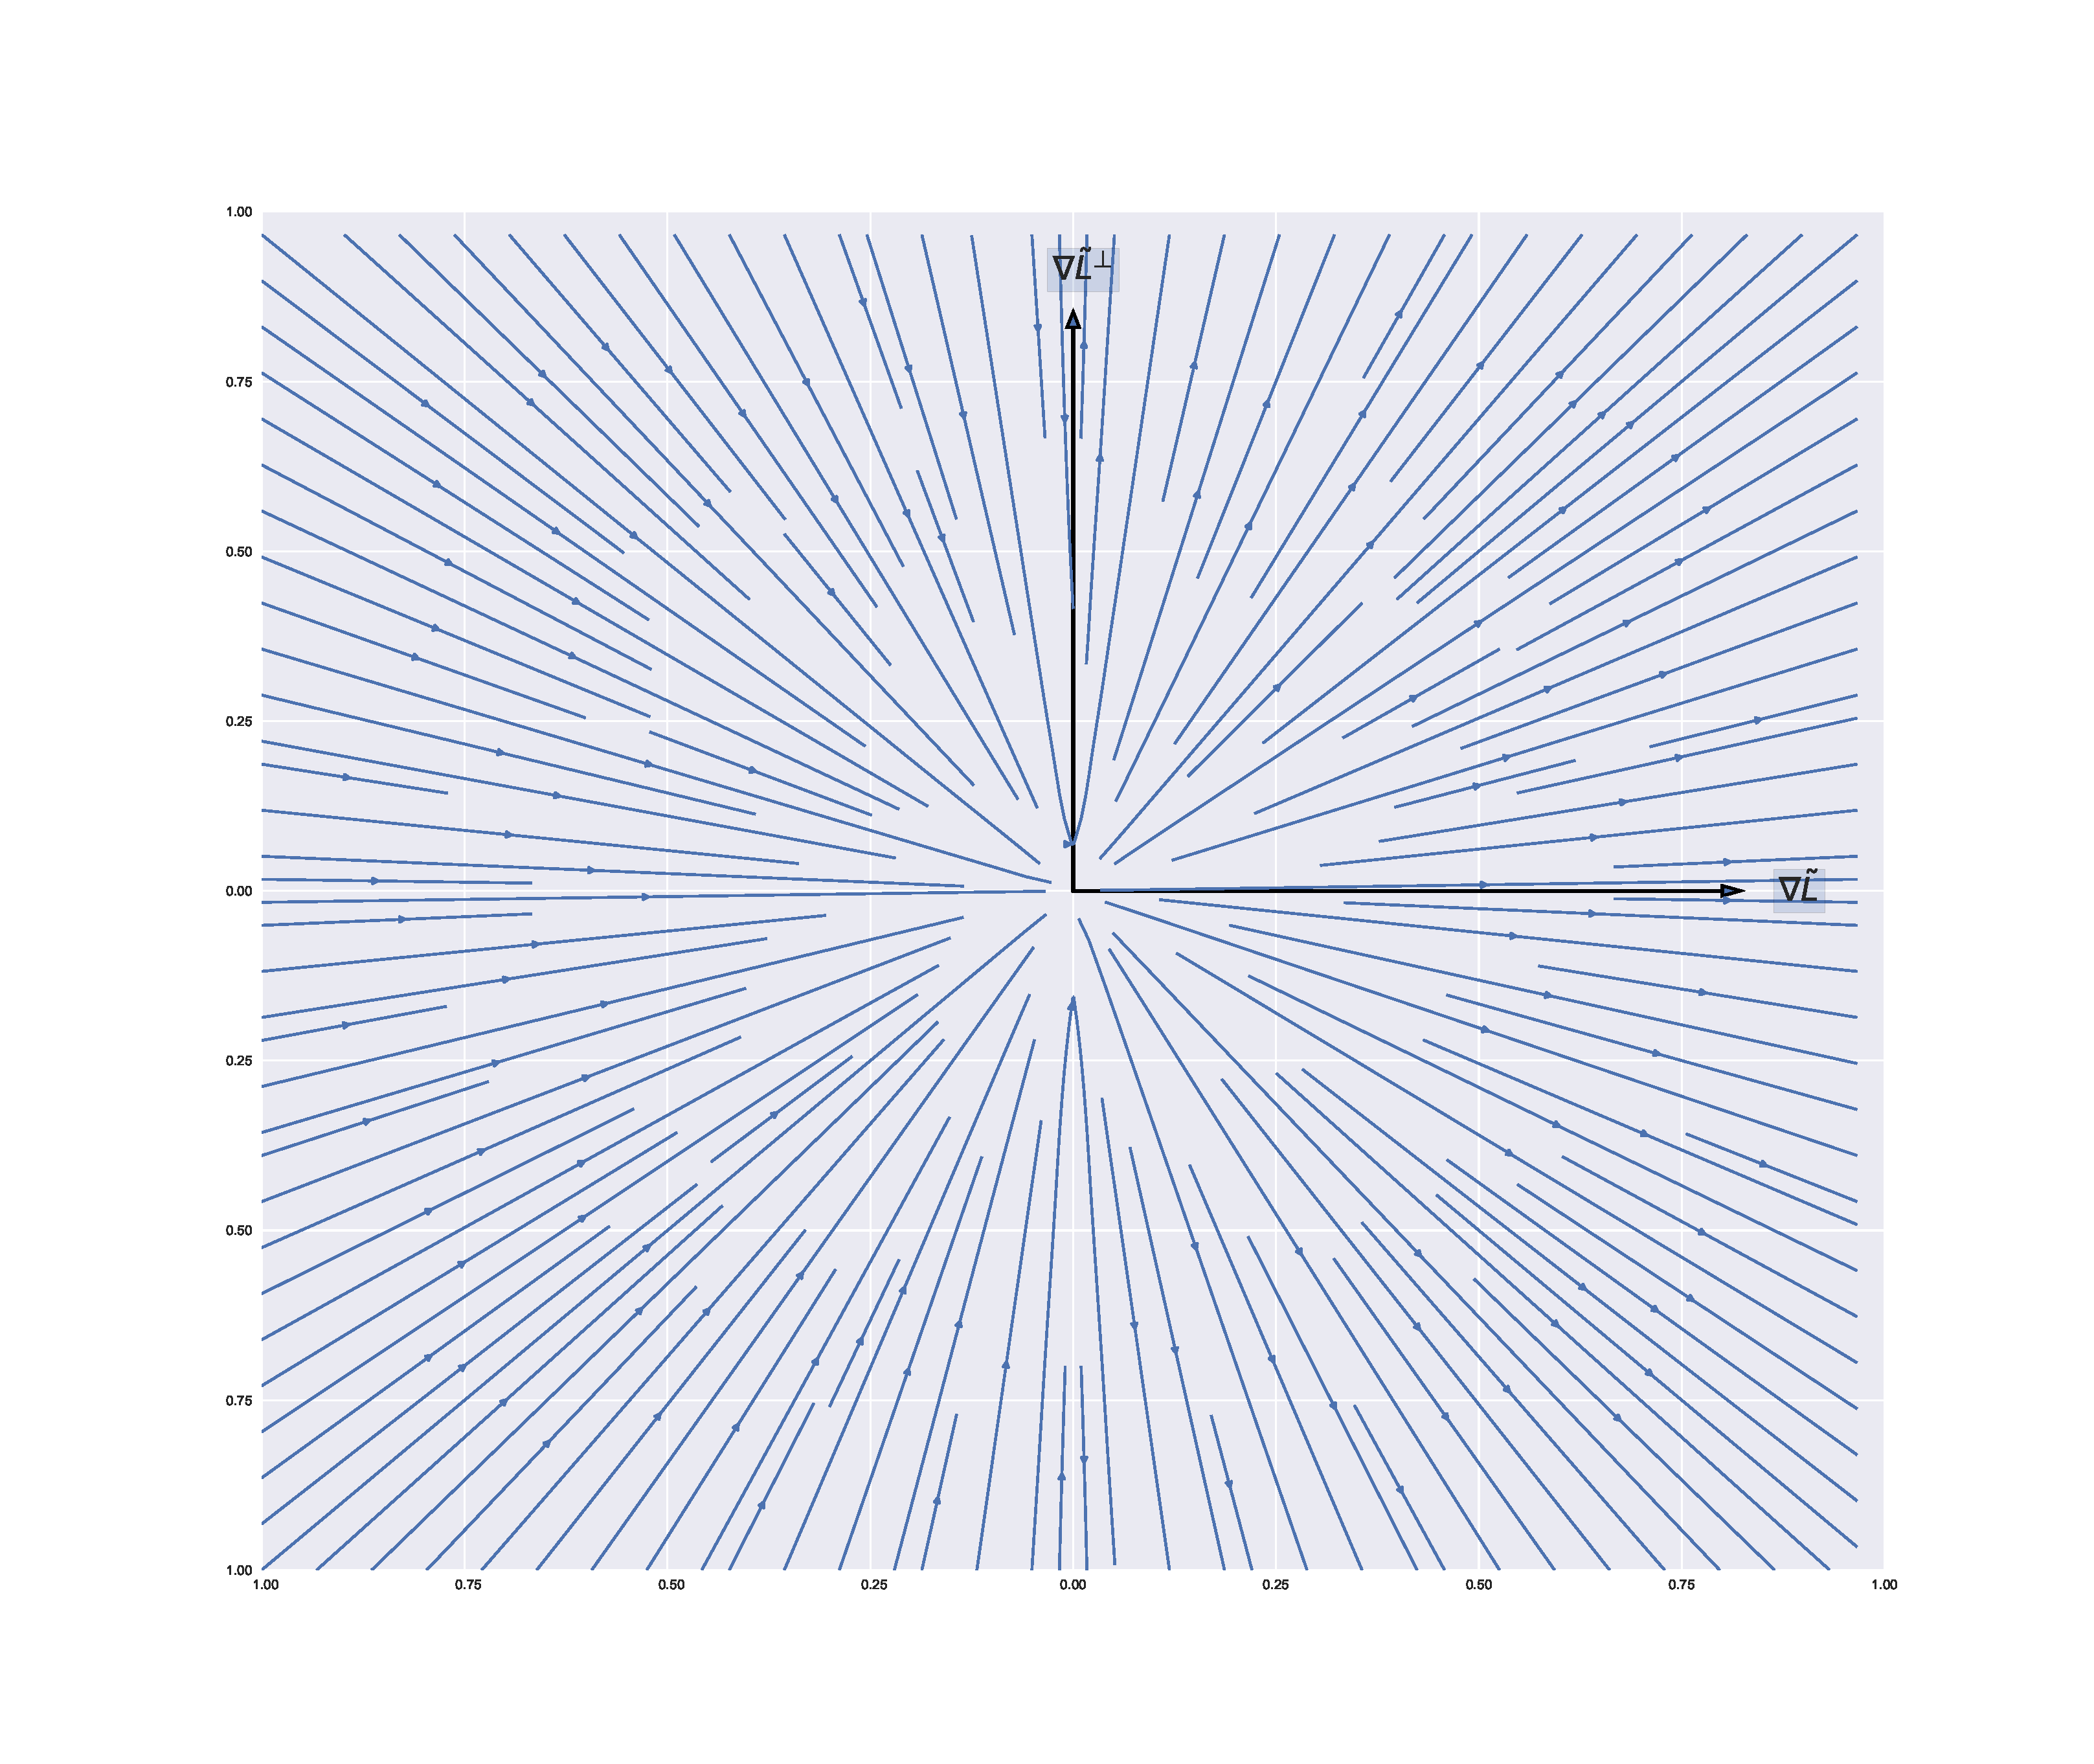
\includegraphics[width=\linewidth]{figures/dynamics_delta_-100.pdf}
    \endminipage\hfill
    % \minipage{0.2\textwidth}
    % 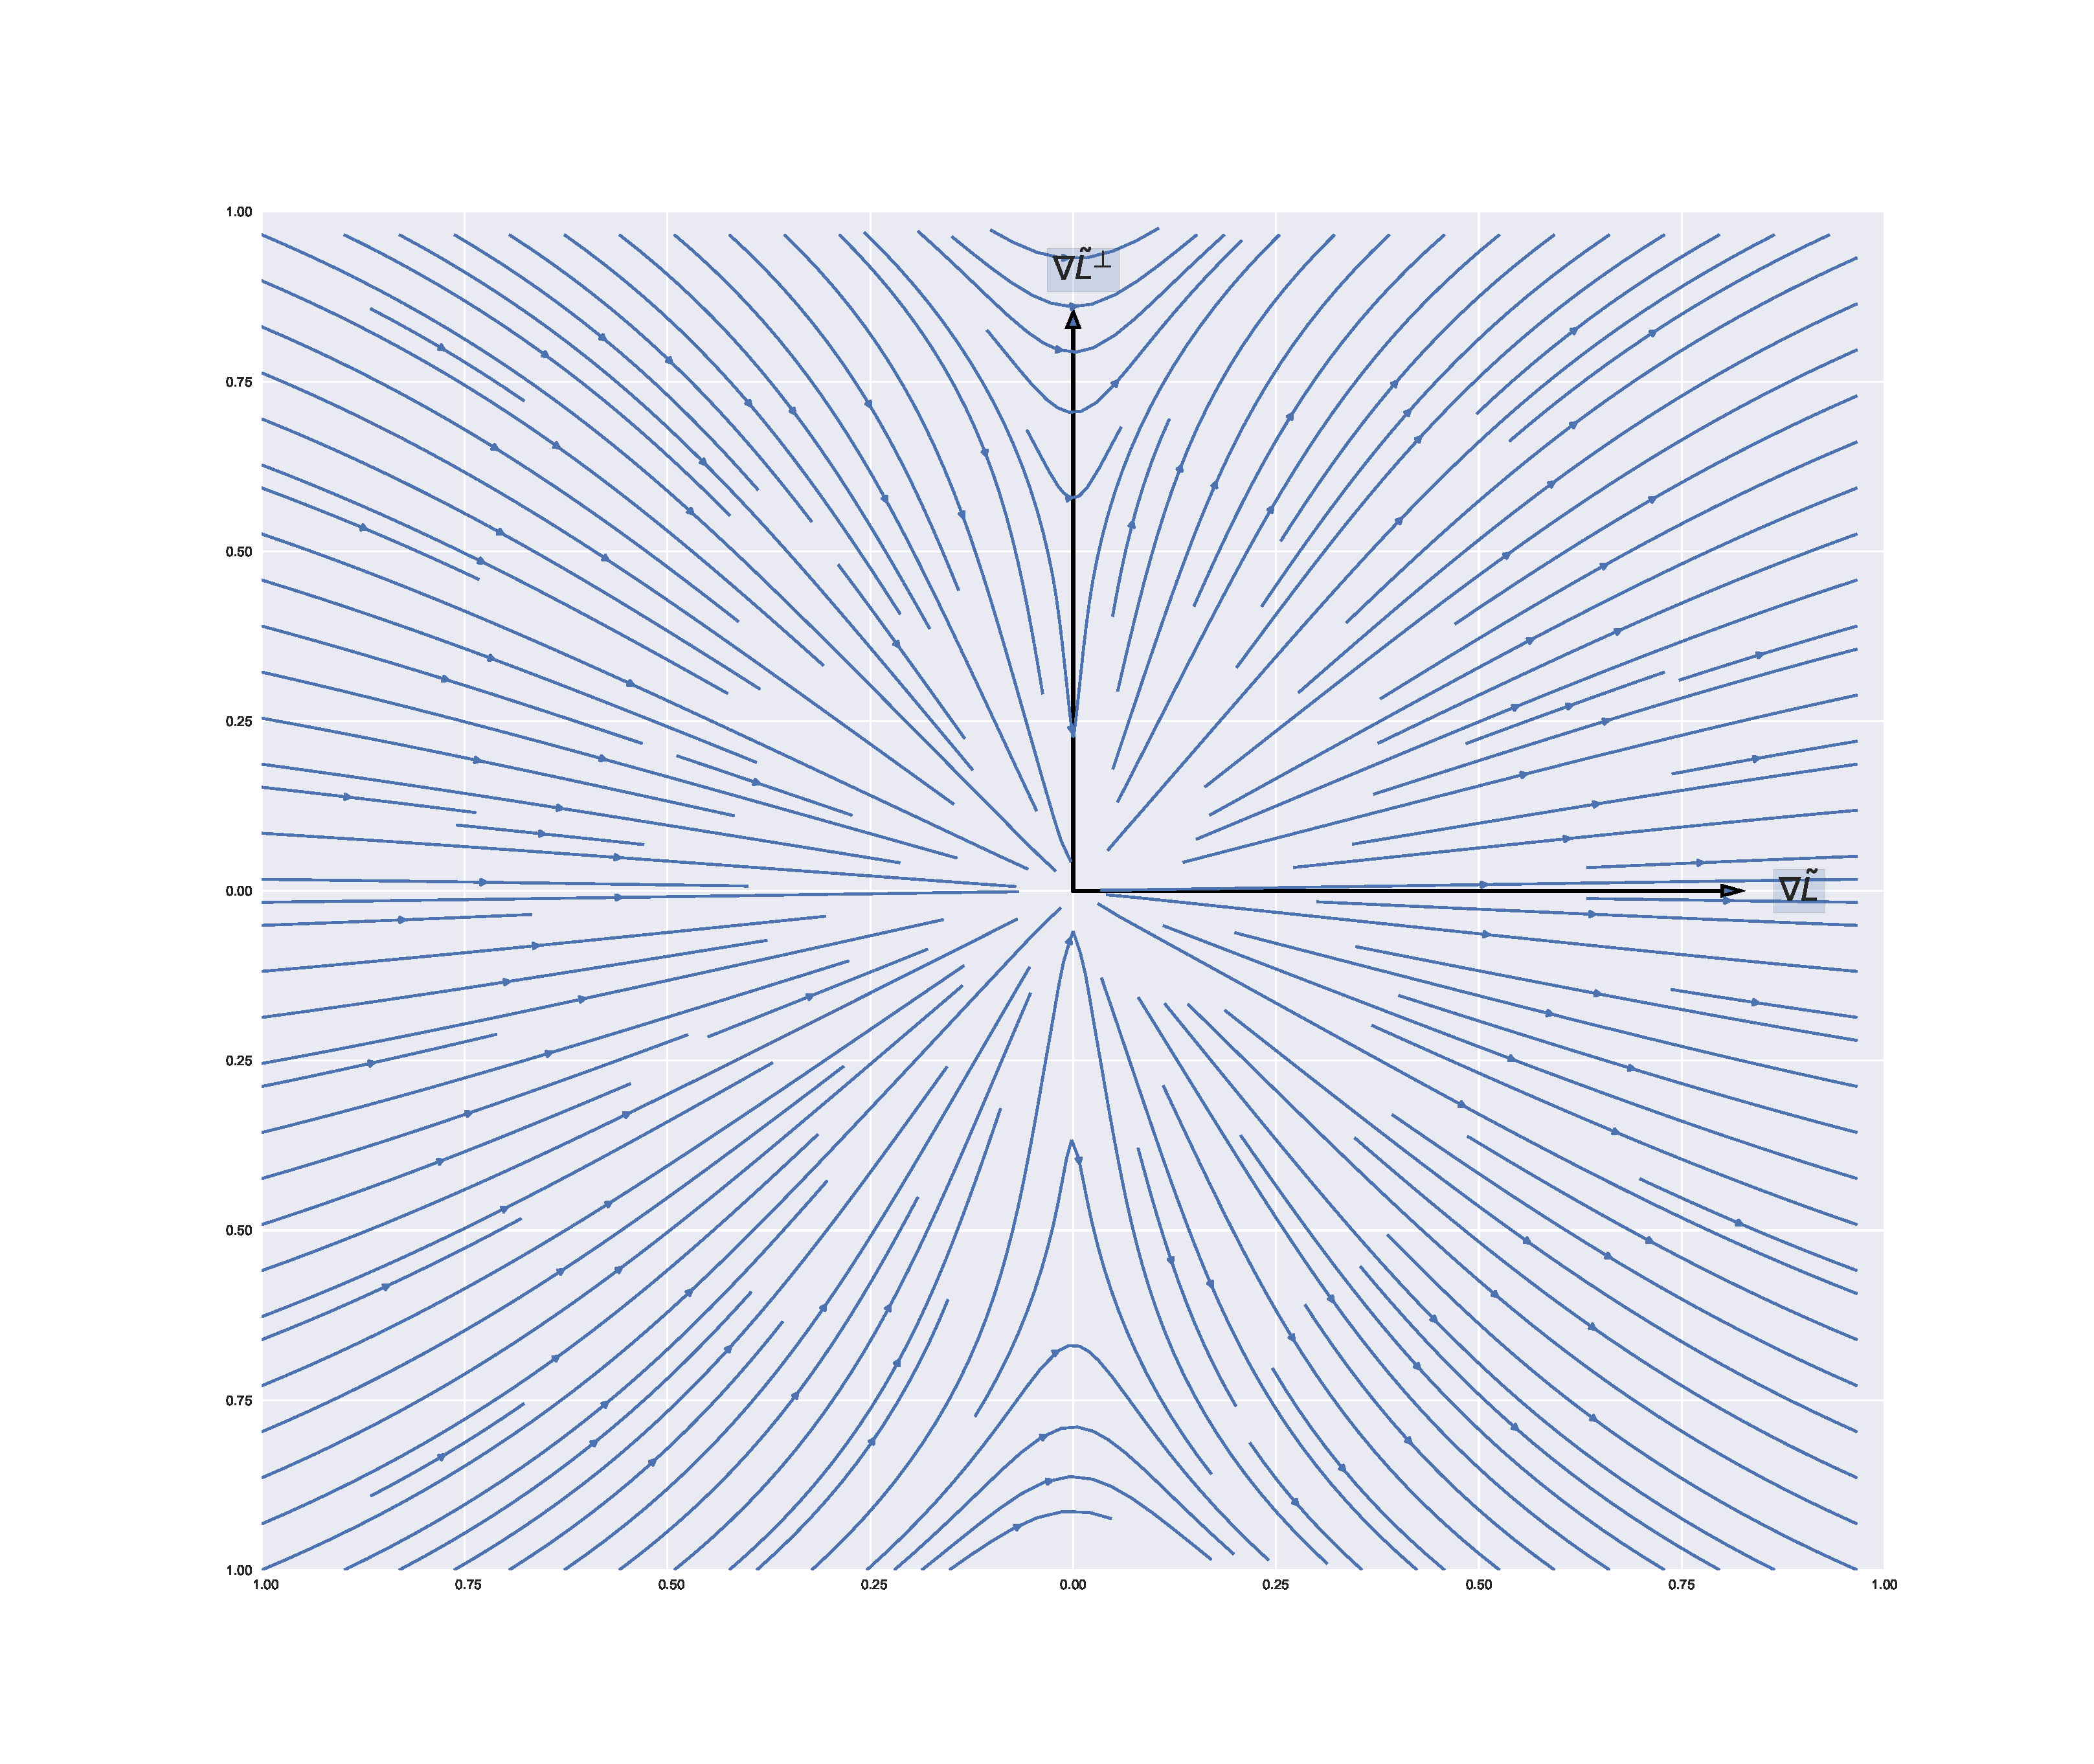
\includegraphics[width=\linewidth]{figures/dynamics_delta_-1.pdf}
    % \endminipage\hfill
    \minipage{0.33\textwidth}
    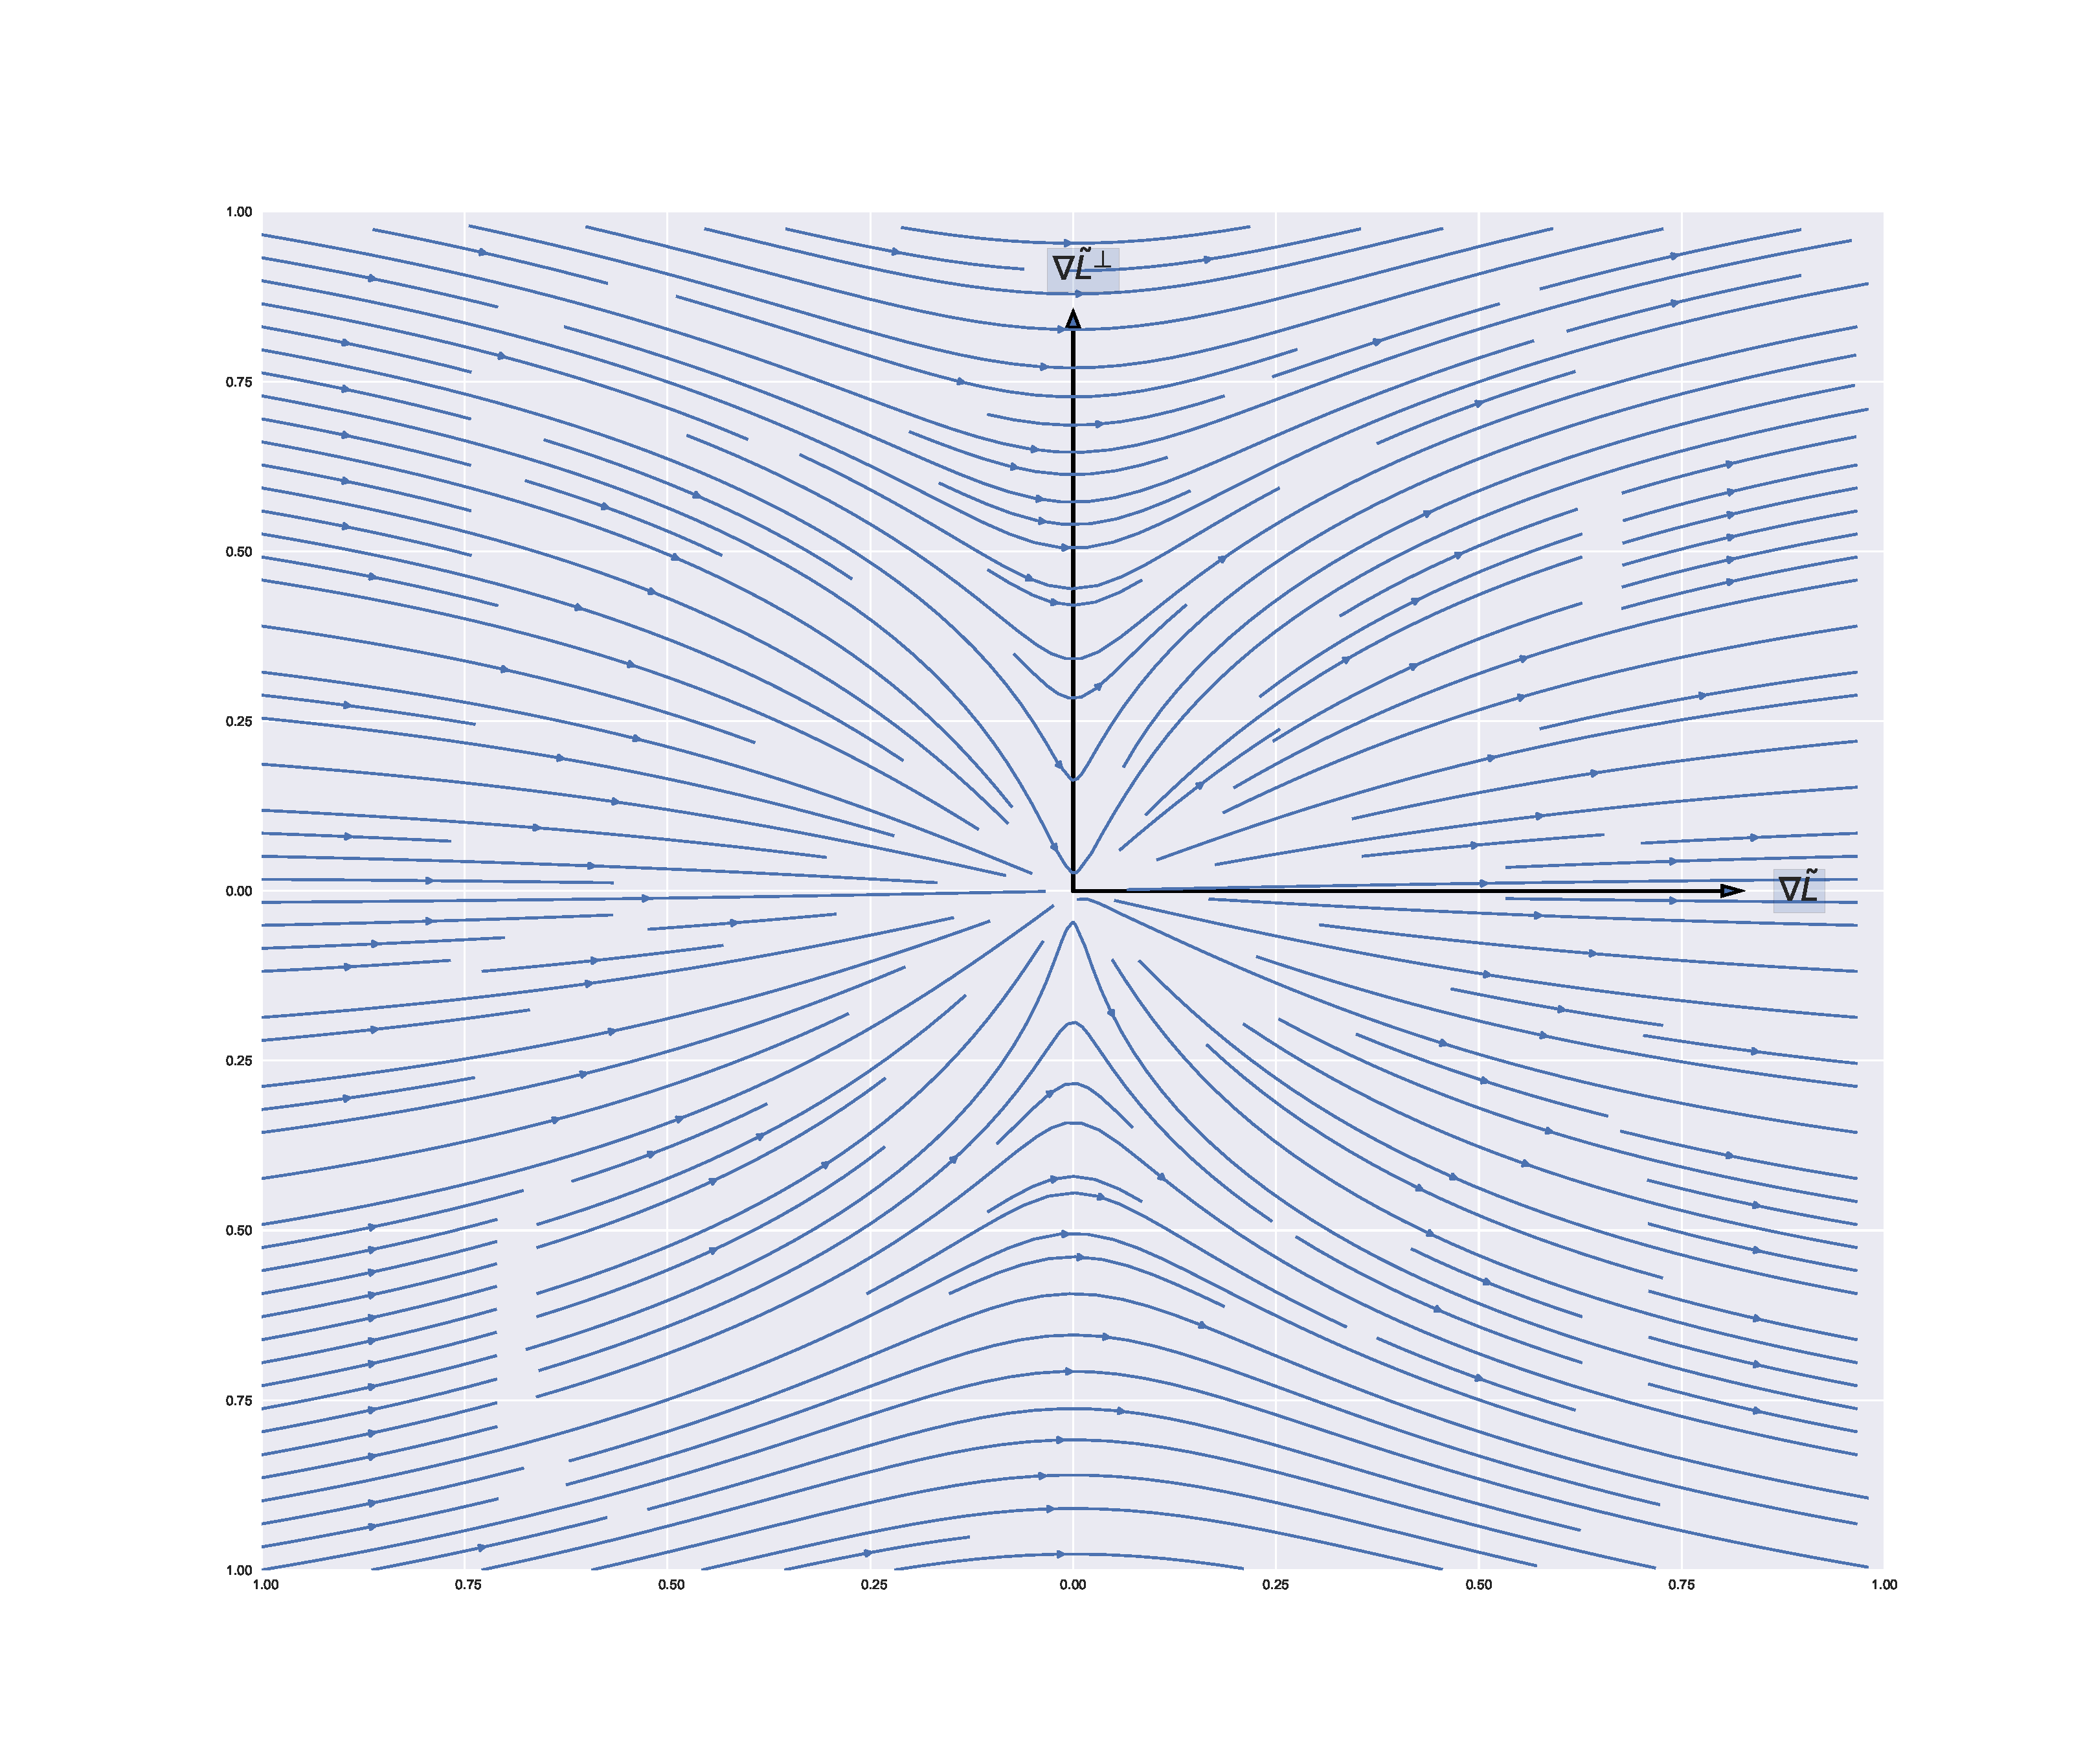
\includegraphics[width=\linewidth]{figures/dynamics_delta_0.pdf}
    \endminipage\hfill
    % \minipage{0.2\textwidth}
    % 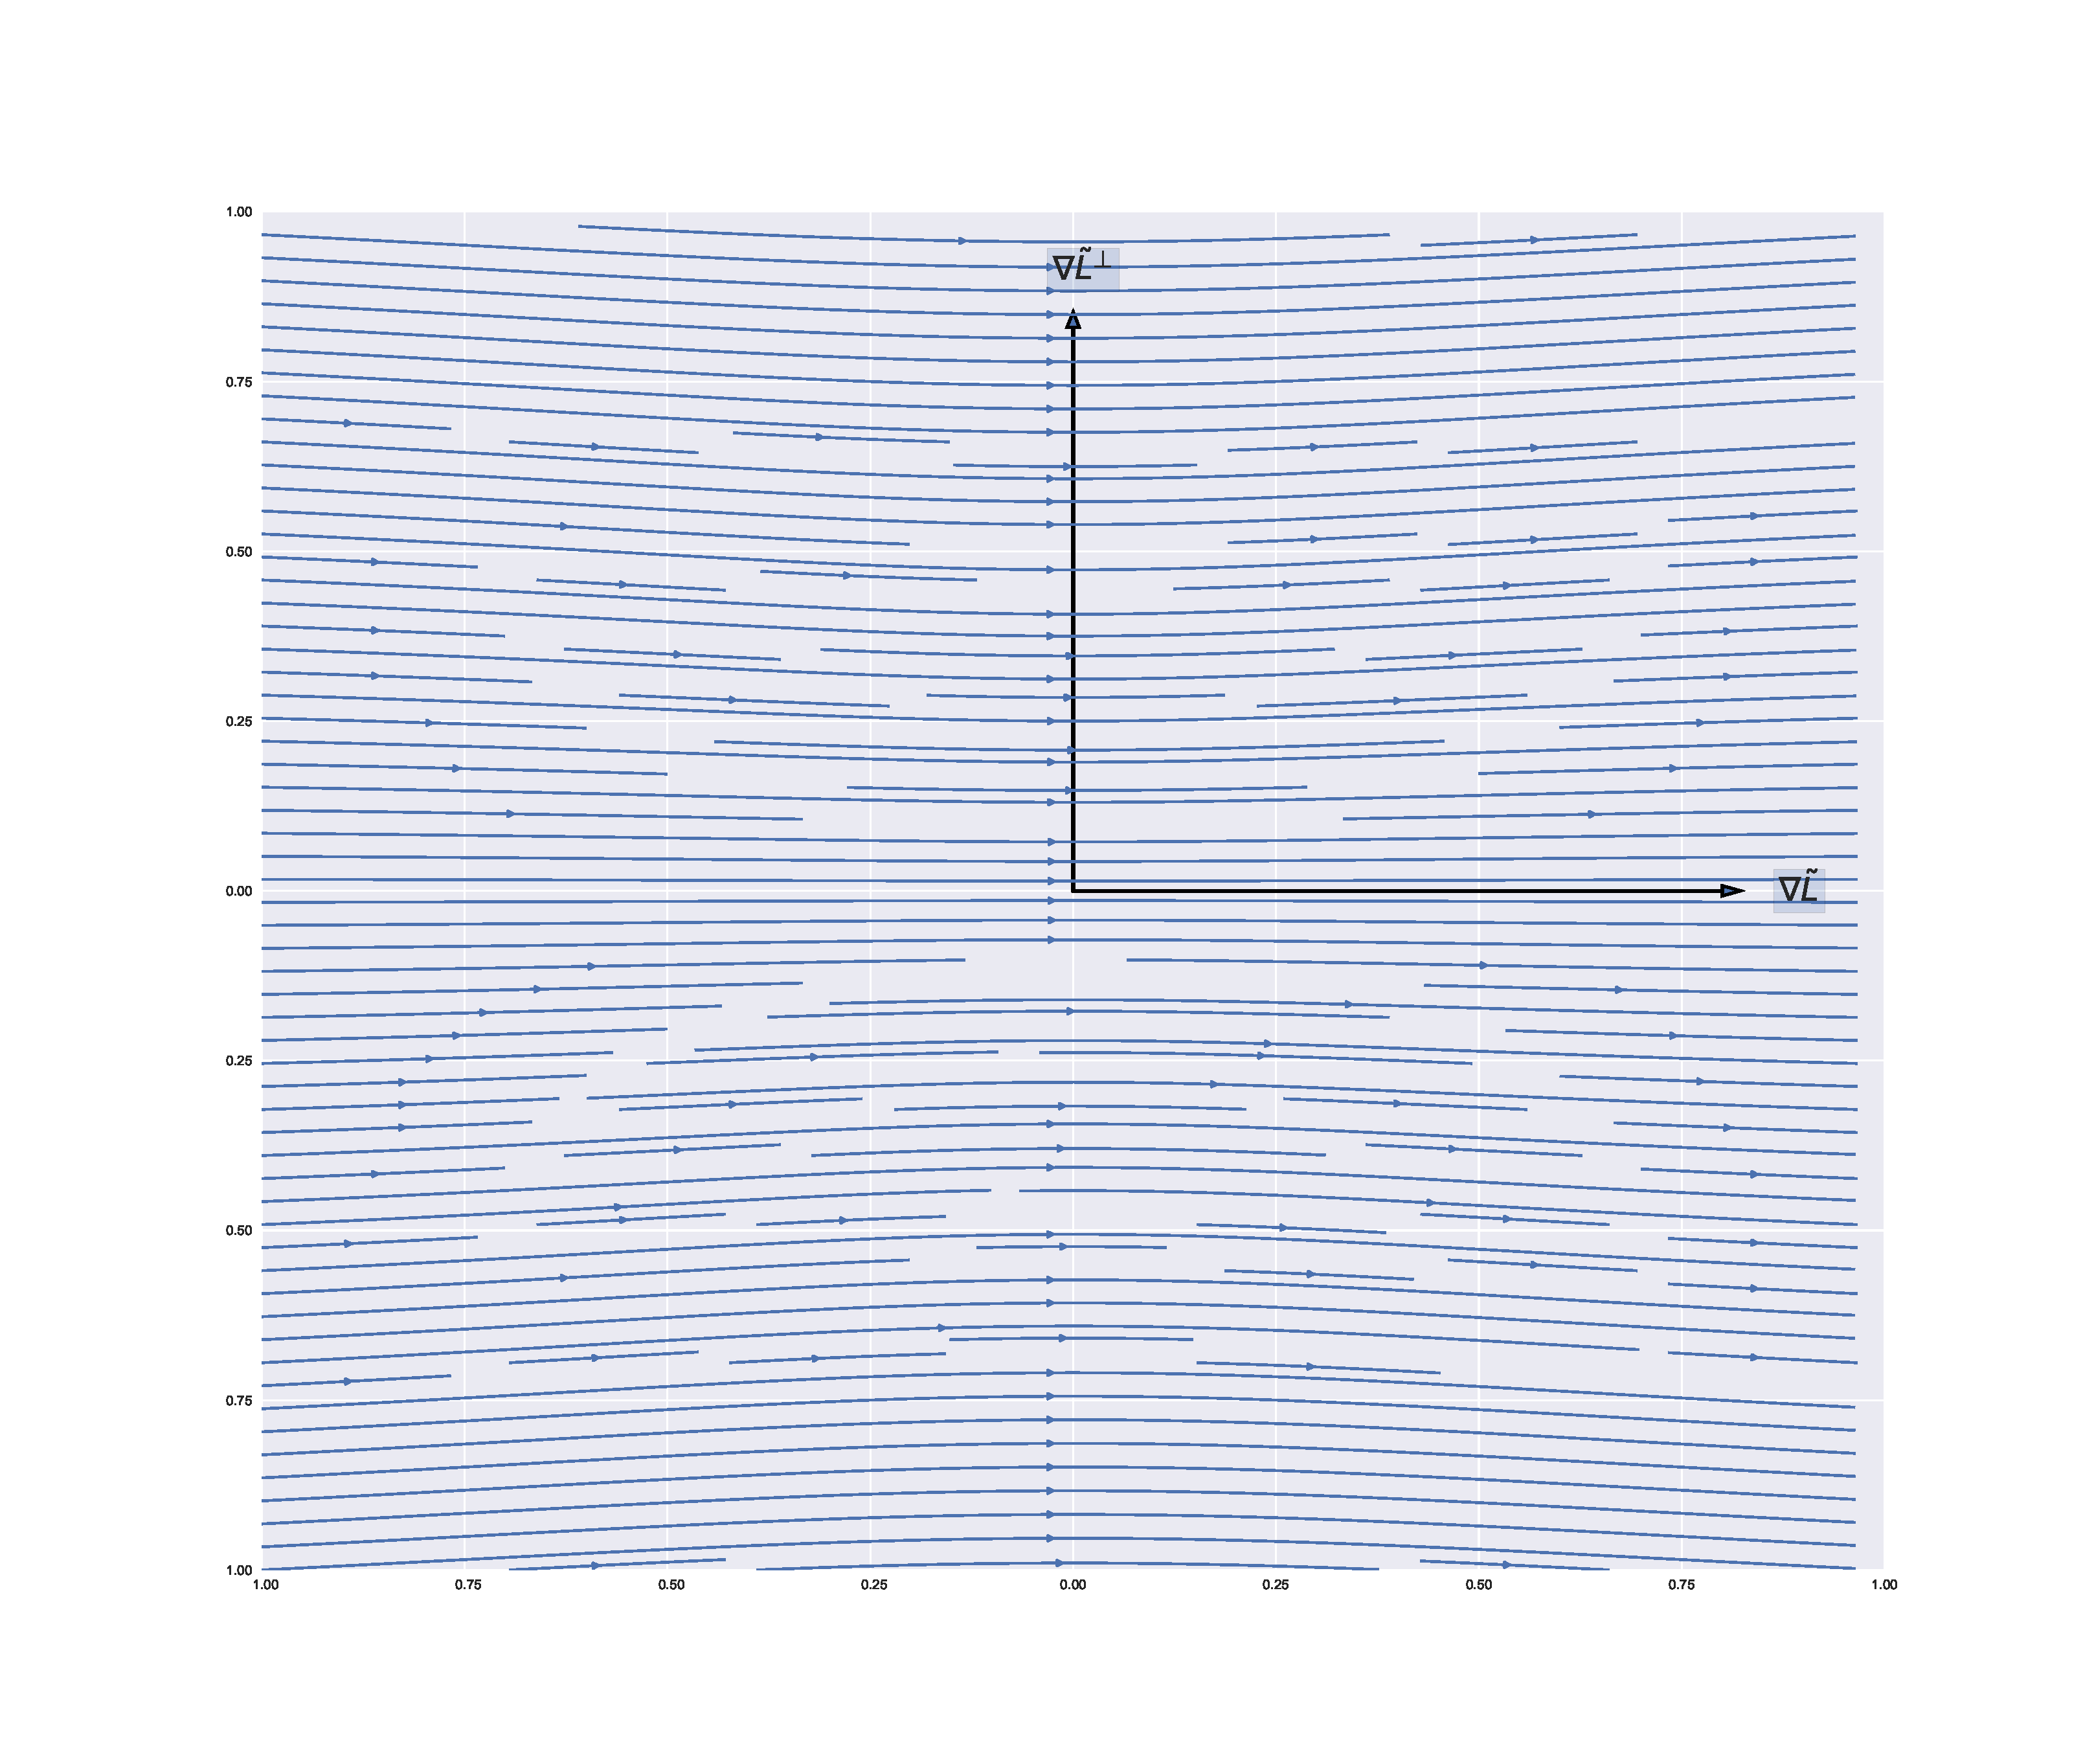
\includegraphics[width=\linewidth]{figures/dynamics_delta_1.pdf}
    % \endminipage\hfill
    \minipage{0.33\textwidth}
    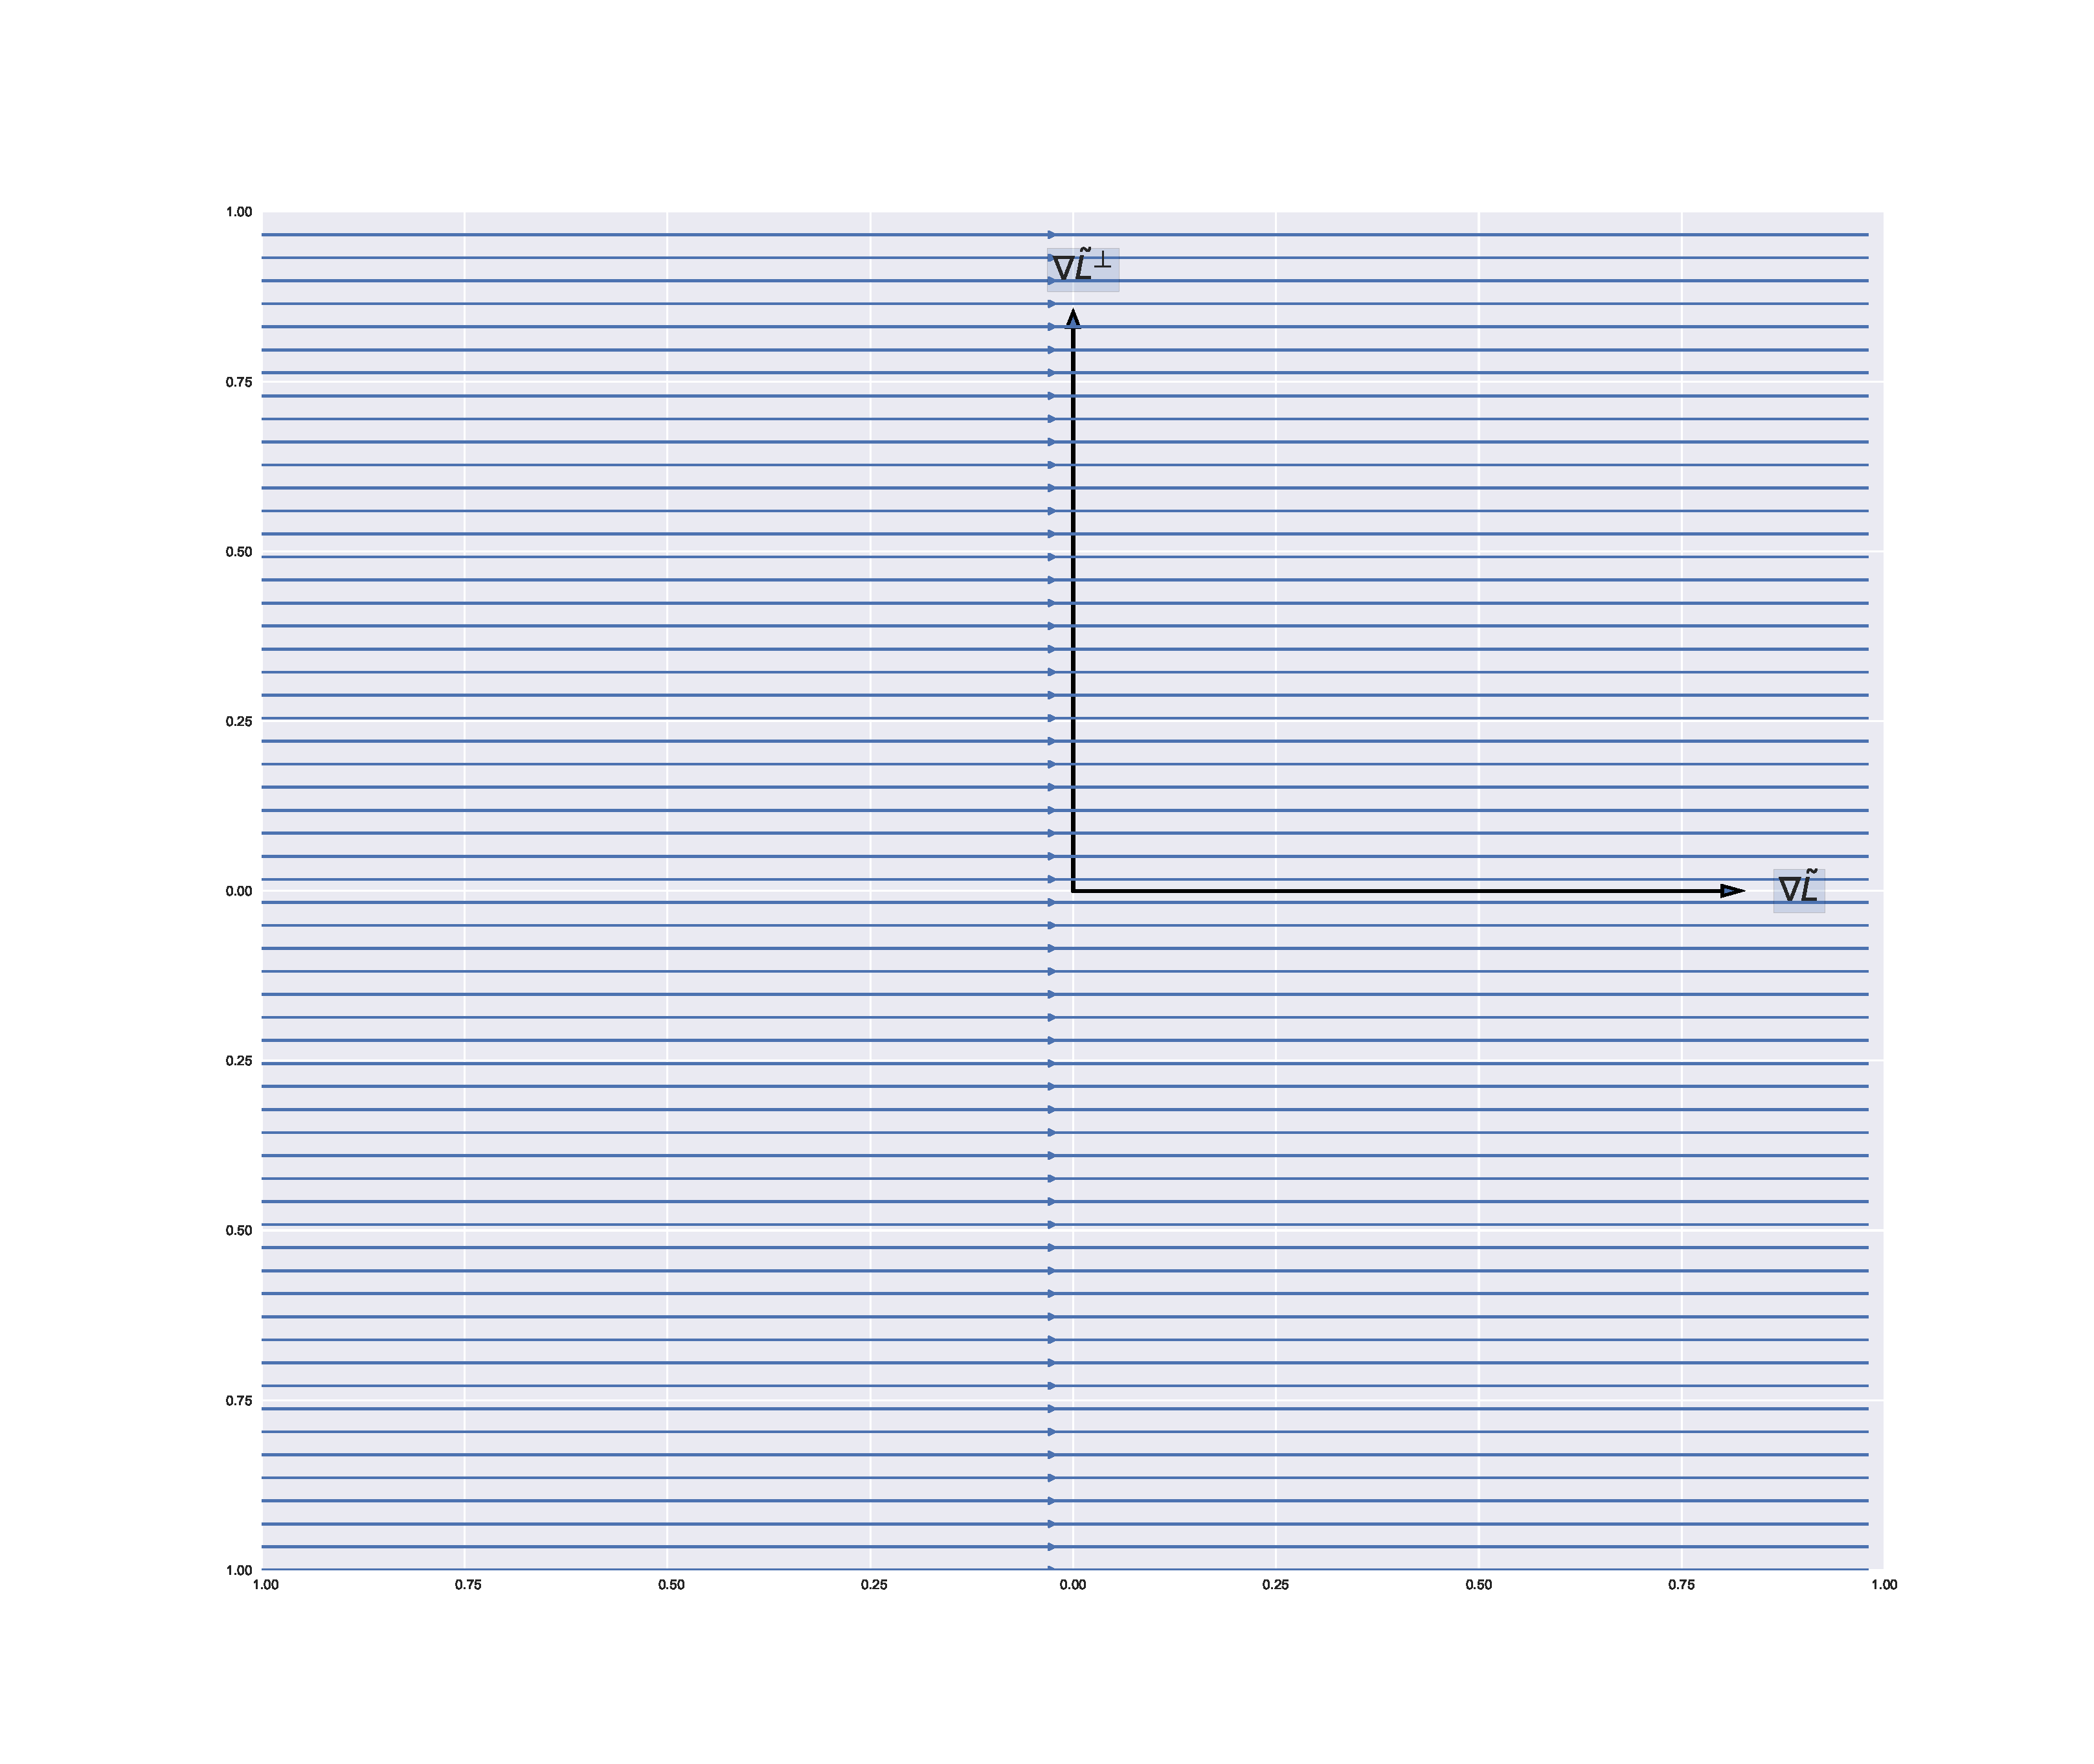
\includegraphics[width=\linewidth]{figures/dynamics_delta_100.pdf}
    \endminipage
    
    \caption{The value of $\delta$ interpolates between different kinds of local trajectories of neurons. The plots are in the coordinate frame $(\nabla \tilde{L}, \nabla \tilde{L}^\bot)$. The left shows $\delta = -100$, in this case, the neurons move radially towards and away from the origin. The middle image shows the trajectories for $\delta = 0$ which has trajectories containing both radial and tangential components. The right image shows the trajectories for $\delta = 100$ which are parallel to the gradient $\nabla \tilde{L}$.}
    \label{fig:my_label}
\end{figure}





